\section{A Series of Tubes - A Tool for Tube Design}

We created a tool which makers can use to create tube-powered interfaces in arbitrary 3D models.  This tool allows designers to brush over the surface of their model to select exterior connection points of their tubes (see Figure \ref{fig:tool-process-interior}) or to import vector art describing the tubes' interior paths (see Figure \ref{fig:tool-process-exterior}).  Once the user's selections are made, we create a complete routing using either the exterior connection point method (A*) or the interior path method (graph edge creation, Euler circuit generation).  We thicken our routing and use a physics-based rod simulation to minimize bending energy of tubes.  We also apply templates where appropriate (e.g., 3D cross-overs for tubes that intersect in the plane).  The resultant routing is subtracted from the original mesh.  The modified mesh can then be 3D printed.

Our tool is implemented as a part of Meshmixer, a consumer mesh editing tool, in C++.

\subsection{Exterior Connection Points}

To create tubes in which the location and shape of exterior connection points matters, we first allow users to select the connection points on the mesh's surface using a brush. Our tool then creates an initial shortest-path routing using A* to estimate the routed distance between points.  This routing is used to create a rod; we run physics-based simulation steps on the rod to minimize its bending energy (and thereby minimize the bend radius of the tubes).

\begin{figure}[h!]
\centering
    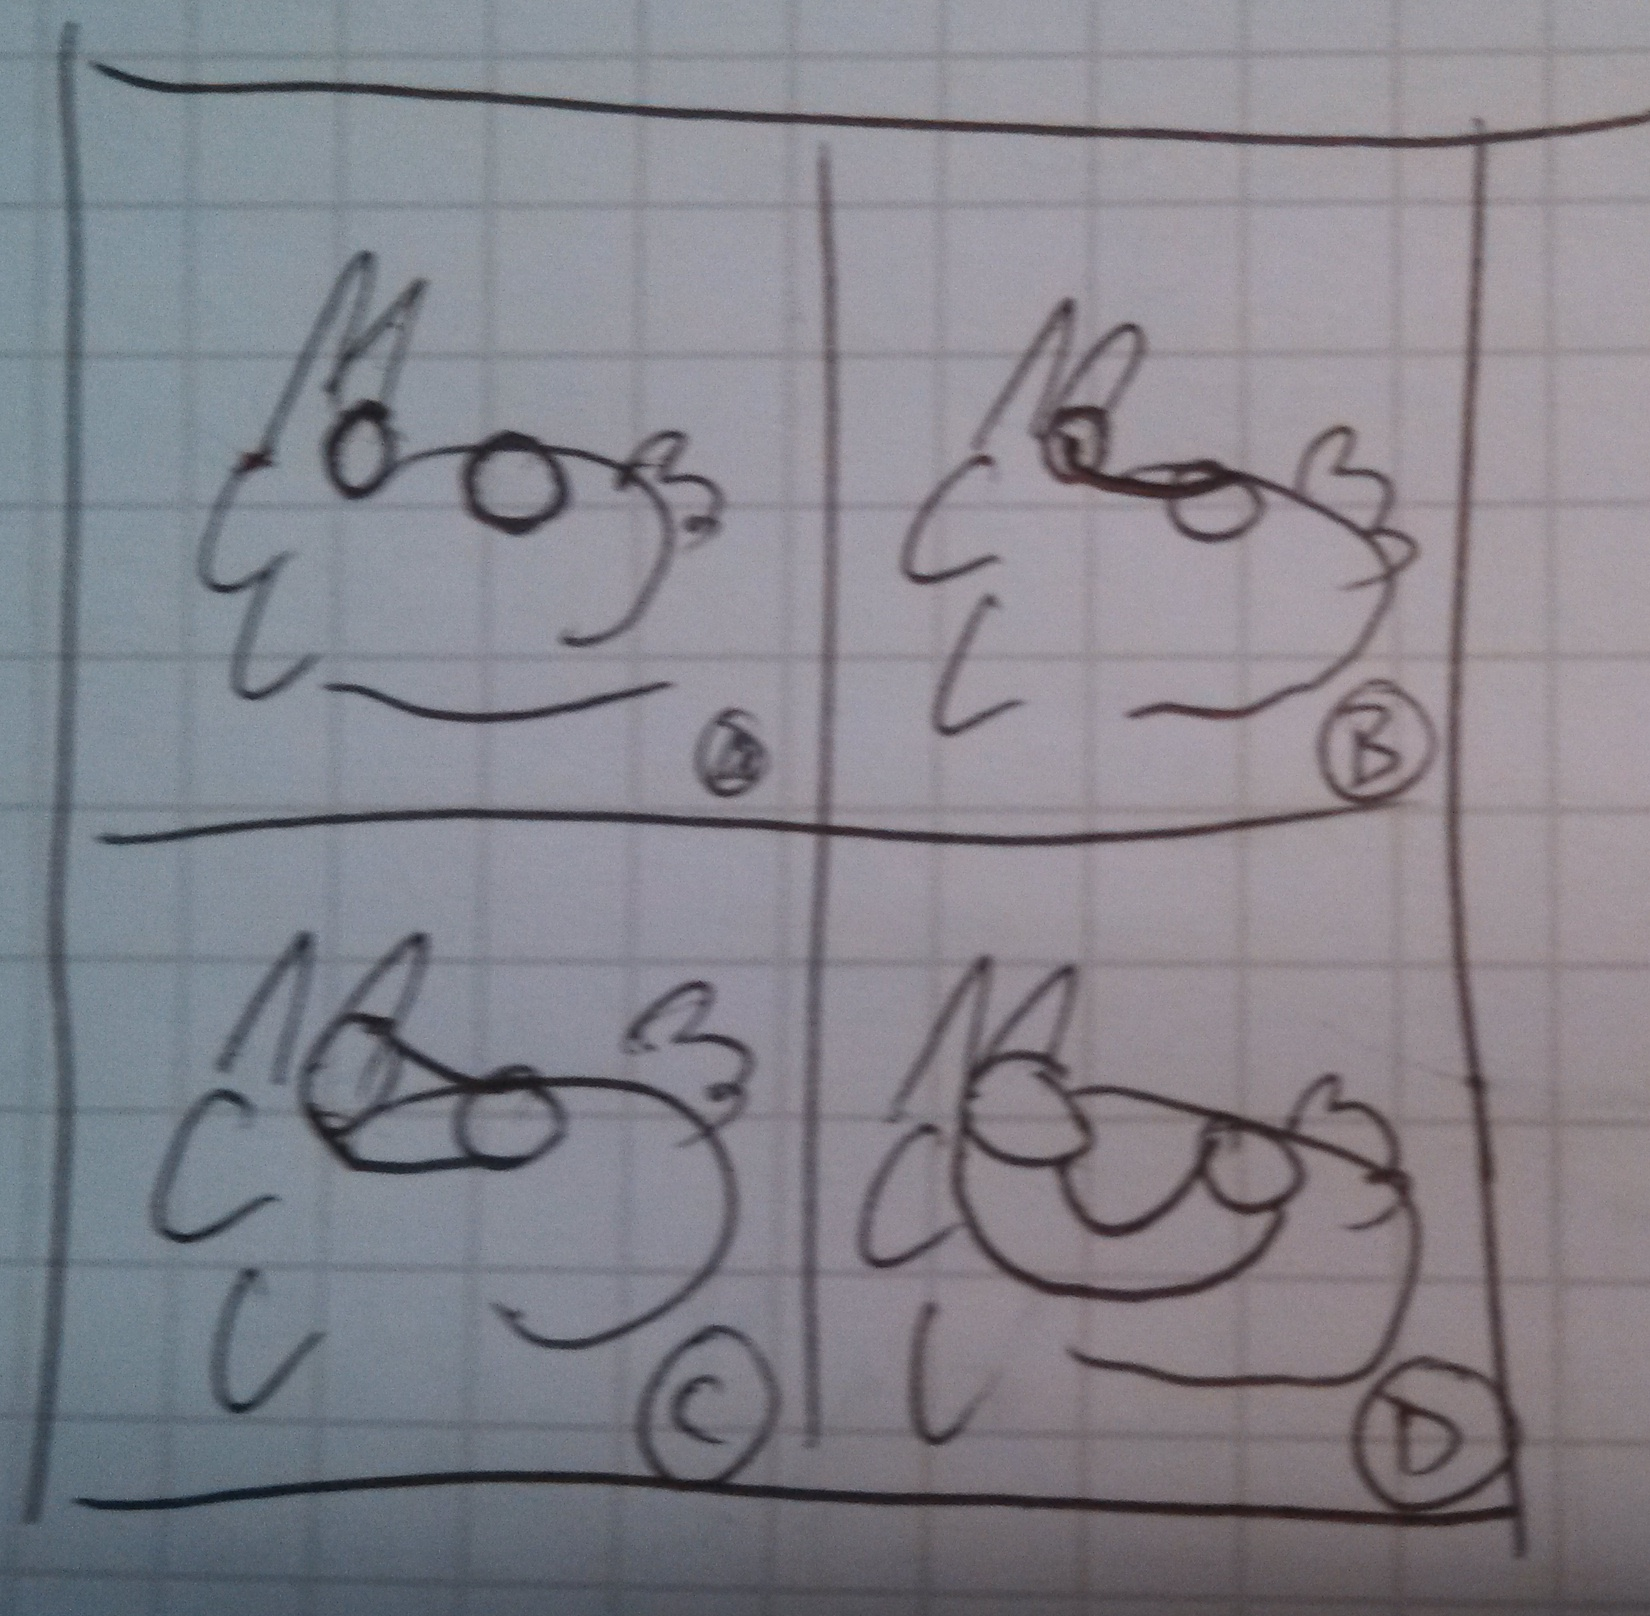
\includegraphics[width=3.4in]{figures/placeholder/exterior.jpg}
\caption{An example mesh with exterior connection points selected.  The initial A* routing is drawn in {\color{red}red}, and in {\color{tovi}green} is our physically-based rod after simulation.}
\label{fig:tool-process-exterior}
\end{figure}

\subsubsection{Routing}

Our basic first-pass routing algorithm uses the A* routing algorithm \cite{Hart-Astar}.  The path cost in our implementation is based only on shortest distance between the starting and ending points, without weighting for distance from the surface.  We only permit the routing within the voxel grid of the mesh: i.e., the routing is not permitted to traverse through space outside the mesh itself.

Given this initial routing, we create a rod of slightly longer proportional length.  The rod must be longer, as the A* routing can follow the mesh boundaries and the rod requires extra length to be pushed away from the mesh surface.  While we do not have a theoretical basis for this proportional increase, \valkyrie{yet.  what might it be related to?  we can test how much of the A* path is outside the model, and how much is inside; further we can consider the distance from the A* path that is outside the model to the surface.  I think there's a good way to do this.  It might even just mean iteratively changing the rod length until we get something reasonably short and also smooth.  we can also return to the A* that I wrote which finds a routing through the mesh that respects its boundaries; this would get us closer to what we need for length in the first place.}, we have found 1.15 to be a reasonable multiplier in practice.  A too-long rod is forced to kink and expand further than necessary inside the model, while a too-short rod must be stretched, leading to non-smooth bending.

Physical Simulation : 

How does it actually work? \valkyrie{Ryan?}

Bend Minimization

In order to force our simulated rods away from the surface of the mesh, we create ``wind'' pushing inward from the exterior of the mesh.  This wind pushes the tube away from the surface.

\subsubsection{Tubes with Multiple Endpoints}

To allow designers to create tubes with multiple endpoints (like the star topologies in Figure \ref{fig:toys}), we ....???? \valkyrie{create 0-size mesh points in the center of the object, to which we attach one end of every tube?}

\subsection{Designing Interior Paths}

A user can import a vector graphics file (such as SVG) describing the path she desires for her tubes.  We create a graph based on this input data, then add edges to make it connected and semi-Eulerian.  We create an Euler tour on the modified graph, and thicken the path to create tubes.  3D templates are used to resolve tube crossings in the plane.

\begin{figure}[h!]
\centering
    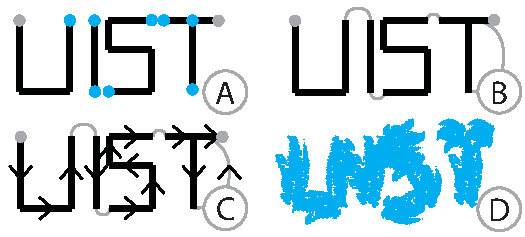
\includegraphics[width=3.4in]{figures/interior.pdf}
\caption{An input vector graphics file with the points which cannot be tubed as drawn highlighted in {\color{blue}blue} (a).  The connected graph created by our software (b) and the resulting Euler circuit (c) permit creation of a novel neon sign (d).}
\label{fig:tool-process-interior}
\end{figure}

\subsubsection{Routing}
The interior path routing problem is a version of the Chinese Postman Problem\footnote{The CPP is also known as the route inspection problem: \url{http://en.wikipedia.org/wiki/Route_inspection_problem}}, in which we wish to traverse all edges of the graph described in the user's input with a single Euler circuit, much as a postman needs to walk along every road at least once to deliver mail.  We call our relaxation the Spiderman Postman Problem: we allow the creation of non-existing paths (i.e., the postman may traverse buildings in addition to roads).  If inputted path components are disconnected, we must create edges that connect them; additionally we can create new edges connecting odd-degree vertices rather than simply retracing existing edges.  In the final artifact, all created edges will be blocked out by dark material so the inserted medium is not visible (see Figure \ref{fig:tool-process-interior}).

We want a semi-Eulerian graph (i.e., we want a graph in which every vertex but two have even degree) so that the desired medium can be inserted, traverse every edge, and exit the graph at a different vertex.  Let $G=(V,E_0)$ s.t. $\forall e \in E_0, weight(e)=0, start \in V $ the start point $end \in V$ the end point.  Let $e_{temp} = (start, end)$, $E' = E + e_{temp}$.

We need to connect disconnected subgraphs in $G$.  Let $G_{dis} = \{G_1, G_2, ... G_n\} \in G$ s.t. $\cup{\{G_i \in G_{dis}\}} = G$ and $G_i \cap G_j  = \{ \} \forall G_i, G_j \in G_{dis}, i\neq j$ be disconnected subgraphs in G.  Create $E_{conn} = \{e = (u, v), u \in G_i, degree(u)\%2 = 1, v \in G_j, degree(v) \%2 = 1 i \neq j, weight(e) = distance(u, v)\}$ be the set of all edges connecting odd-degree points in two distinct disconnected subgraphs.  To keep only the most desirable edges in $E_{conn}$, contract each subgraph $G_i$ to a single point $u_i$ with the shortest outgoing edges to each other subgraph: $E_{conn} = \cup_{G_i \in G_{dis}} \{e=(u_i, v), v \in G_j,$ s.t. $\forall E_{conn} \ni e_k = (u, v), u \in G_i, v \in G_j, weight(e_k) \geq weight(e)\}$.  Sort $E_{conn}$ s.t. $E_{conn} = \{e_1, e_2, ... e_n\}, weight(e_1) \leq weight(e_2) \leq \ldots \leq weight(e_n)$.

Let $E_{conn-min} = \{ \}$.  Beginning with $e_1$, add the first edge $e_i \in E_{conn}$ to $E_{conn-min}$.  Then let $E_{dupe} = \{ e = (u, v) \in E_{conn}$ s.t. $u$  is reachable from $v$ along edges $E' \cup E_{conn-min}$.  Let $E_{conn} = E_{conn} \setminus E_{dupe}$.  Repeat until $E_{conn} = \{ \}$.  Let $E' = E' \cup E_{conn-min}$.

At this stage, we want an Eulerian graph: i.e., we need every vertex to be of even degree.  Let $V_{odd} = \{ v \in V$ s.t. $degree(v) \% 2 = 1 \}$.  Create $E_{circuit} = V_{odd} \times V_{odd}$, s.t. $\forall e=(u,v) \in E_{circuit}, weight(e) = distance(u, v)$.  Find minimum matching $E_{circuit-min} \subseteq E_{circuit}$.  Let $E' = E \cup E_{circuit-min}$.

Now to remove our temporary edge and make the graph semi-Eulerian instead of Eulerian, let $E' = E' \setminus e_{temp}$.

\valkyrie{does the proof of this theorem belong in the paper, or in the appendix?  we can push it back there if need be, although it's not super long.}
\begin{theorem}
 $G' = (V, E')$ is a connected, semi-Eulerian graph for which $E \subseteq E'$. \valkyrie{why is there such a huge space after this paragraph?}
\end{theorem}
\begin{proof}
$E \subseteq E'$ : we never remove edges from $E$ in our algorithm.  $\therefore E \subseteq E'$.

$G' = (V, E')$ is connected : if $G'$ is not connected, $\exists G_i = (V_i, E_i) \subset G', u \in V_i, v\in V \setminus V_i$ s.t. $u$ is not reachable from $v$.  $G_i \not\in G_{dis}$, because we create edges connecting $G_j, G_k \forall G_j, G_k \in G_{dis}$ and only remove an edge $e_{dupe} = (u, v)$ from $E_{conn}$ once we determine that $u$ is reachable from $v$ along edges $E' \cup E_{conn-min}$.  $\therefore G_i \not\in G_{dis}$.  This implies that $G_i$ was not initially disconnected from $G$, because by definition $G_{dis}$ is the set of all disconnected subgraphs of $G$.  We cannot have disconnected $G_i$ from $G$ because $E \subseteq E'$.  Thus, a contradiction.  $\therefore G' = (V, E')$ is connected.

$G' = (V, E')$ is semi-Eulerian : Each edge $e$ in our minimum weight matching connects a unique pair of vertices $v_i, v_j \in V_{odd}$ by the definition of minimum weight matching.  Each edge $e = (v_i, v_j) \in E_{circuit-min}$ adds one to the degree of $v_i$ and $v_j$, causing them to be of even degree. $|V_{odd}| \% 2 = 0$ by the handshake lemma, $\therefore$ all edges can be paired.  When we remove $e_{temp} = (start, end)$ from $E'$, we cause those vertices, which were of even degree by the above process, to be of odd degree.  Thus, all vertices except $start$ and $end$ (which are of odd degree) are of even degree.  $\therefore G'$ is semi-Eulerian.
\end{proof}

We believe that a lower total weight matching is possible by connecting components and ensuring edge degree evenness together in a global process, however it this not crucial for our purposes.

Once we have a semi-Eulerian graph, we need to create an Euler tour.  An Euler tour is a path that touches every edge once, beginning and ending at the two nodes of odd degree: in this case, those are the user-selected start and end nodes.  We use a weighted modification of Fleury's algorithm\footnote{\url{http://en.wikipedia.org/wiki/Eulerian_path\#Fleury.27s_algorithm}} for this, where instead of randomly selecting from non-bridge paths at each node, we select the path which turns the least from the most recent path (i.e., we prefer to pass straight through a node, if possible).  This minimizes turns in the final artifact, which eases support material removal and assembly.

\begin{figure}[h!]
\centering
    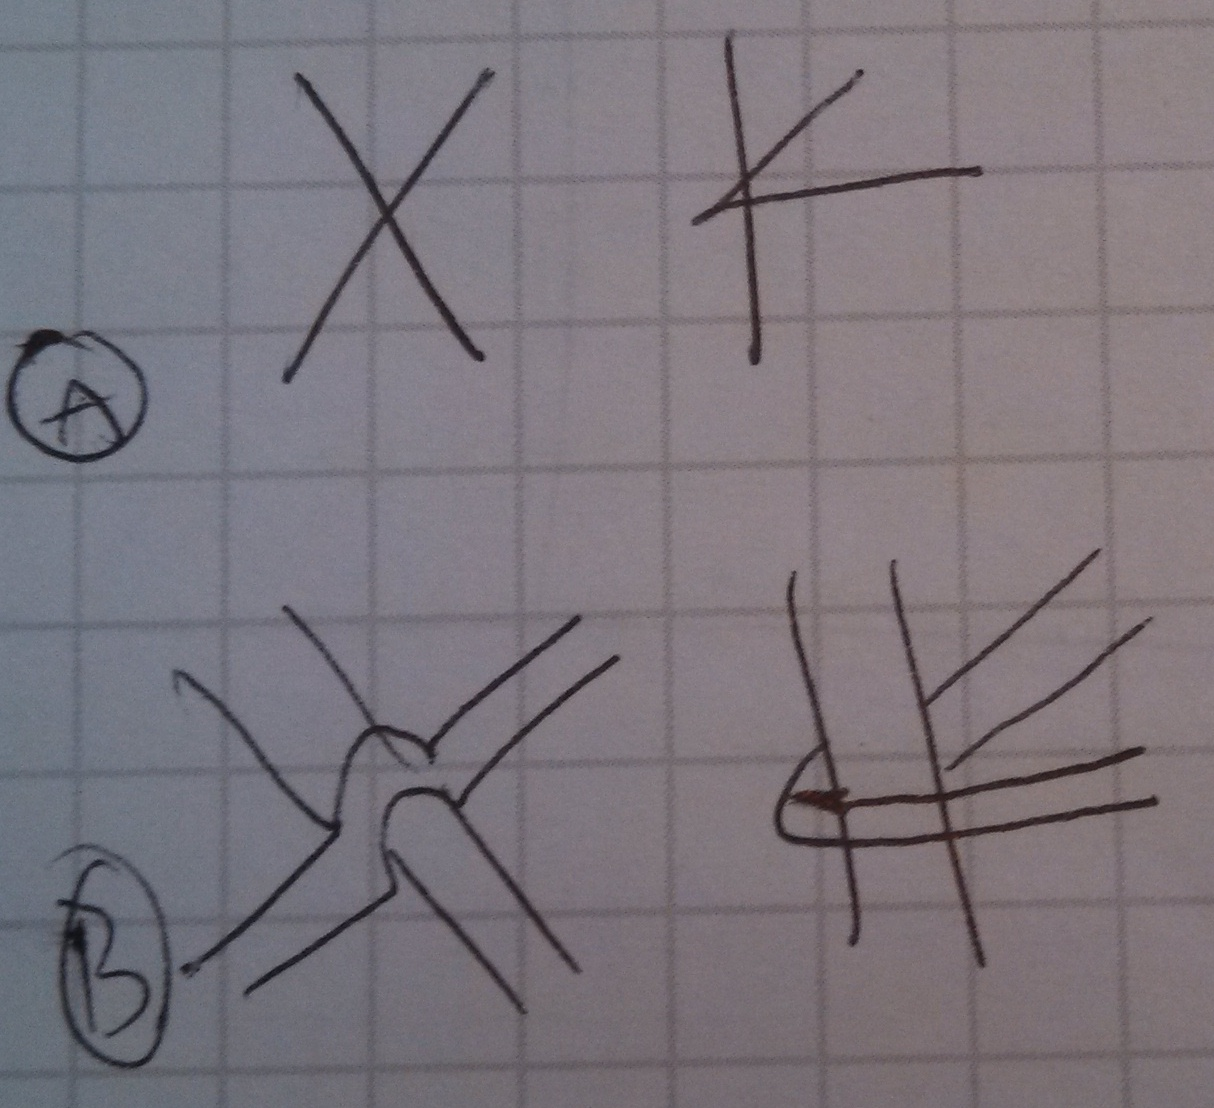
\includegraphics[width=3.4in]{figures/placeholder/templates.jpg}
\caption{When edges intersect in the plane (a), we match them to the nearest of our several intersection templates (b) to create 3D paths that do not interfere with each other.}
\label{fig:templates}
\end{figure}

\subsubsection{Edges that Intersect in the Plane}
Once we have a tour, we must resolve tubes that intersect in the plane.  Because we have a 3-dimensional canvas in which to work, we can push overlapping paths into the third dimension.

To detect intersecting edges, we \valkyrie{I'm not sure what we do.}.  We also consider edges at nodes with degree $>2$, as these edges are considered to cross.  When intersections have been detected, we match one of several templates to the affected edges (see Figure \ref{fig:templates}) using a nearest neighbors technique.  Our templates are parameterized, so the templates can be modified to accommodate precise intersection characteristics.

\valkyrie{For now, we just let them intersect.  The angel hair EL wire is thin enough that we don't actually care.}

\subsection{Mesh Modification}

How we actually cut stuff and make tubes happen. \valkyrie{Ryan?}  We have to actually respect whatever shapes people drew on the surface in the case of the exterior connection tubes (I mean, ideally, we would do a loft operation here).

\subsection{Fabrication Techniques}

\valkyrie{this section may not be at all important.  I was thinking to use it to talk about different ways you can actually build the tubed things, and also constraints set down by the Makerbot vs. the Objet, but maybe that discussion is best made really short and moved to elsewhere}

\subsubsection{Printing} - different strategies with Objet (all print-in-place) and Makerbot (may need to add things like balloons afterwards).  Ryan just got flexible material, we should see how stretchy it is...!  We could also consider assembleable things that are easier to create using parts that clip together... probably out of scope.

\subsubsection{Hand Tools} - post-fabrication modification is possible using hand tools.  We can mark the surface to show where conduits are and how deep.  I can also use this to test things before spending time printing them using a big ol' block o' plastic.